\documentclass[11pt, english, fleqn, DIV=10, headinclude]{scrartcl}

\usepackage[bibatend, color]{header}

\usepackage{pdflscape}
\usepackage[section]{placeins}

\hypersetup{
    pdftitle=
}

\newcommand\mpi{m_{\piup}}
\newcommand\mpipi{m_{\piup\piup}}

\subject{physics760 Computational Physics}
\title{Analysis of $\piup$-$\piup$ lattice QCD \\ scattering data}
%\subtitle{}
\author{
    Martin Ueding \\ \small{\href{mailto:mu@martin-ueding.de}{mu@martin-ueding.de}}
}

\begin{document}

\maketitle

\begin{abstract}
    Correlation functions of pions that were computed with lattice QCD methods
    are analyzed. The effective masses of single pions and two interacting
    pions are extracted. Using a finite size formula by Lüscher, the S-wave
    scattering length is computed.
\end{abstract}

\tableofcontents

\newpage

\section{Data generation}

Monte Carlo methods can be used to simulate quantum systems. Key pieces are
Feynman's path integral formalism and Euclidean spacetime. In the latter, the metric
tensor $\tens\eta$ has signature $\pm 4$ and the weight factor in the path
integral is $\exp(-S_\text{cl})$ instead of $\exp(\iup S_\text{cl})$; 
$S_\text{cl}$ is the classical action
\parencite[Section~2]{Creutz/Statistical_Approach_QM}. A Monte Carlo algorithm
like the Metropolis algorithm can then be used to generate configurations which
are already distributed by the weight of the classical action. Therefore,
expectational values of observables are simply calculated and averaged over all
available configurations \parencite[(3.7)]{Creutz/Statistical_Approach_QM}.

The group of Andreas Kell, Martin Efferz and Simon Blanke have used this for
the harmonic oscillator in their Computational Physics project this year. I
also did this in my bachelor's thesis last year \parencite{Ueding/Bachelorarbeit}.

For quantum chromodynamics (QCD), the theory of the strong force, this
methodology can be used as well. The action of QCD is used with a hybrid Monte
Carlo algorithm to generate configurations of gauge fields on a four
dimensional lattice. This process is done for several ensembles which differ in
parameters like the quark mass. Ensemble generation takes a lot of computing
time, so the results are made available to download.
% TODO Would be nice to have a location where this could be downloaded.

As with the harmonic oscillator on the lattice, expectation values of
observables can be computed for each configuration of the ensembles and then
averaged (without weight) over all ensembles yielding an estimate for the
observable. Since this uses a field theory, particles of interest can be
created at the beginning of time and annihilated laster on. This way, specific
particle configurations (like $\piup$–$\piup$ scattering) can be examined
without needing to generate new configurations.

Using the correct operators, it is possible to construct correlation functions
which contain information about the energies/masses of the involved particles,
analogously to \parencite[(4.14)]{Creutz/Statistical_Approach_QM} for the
harmonic oscillator. I was given those correlation functions to analyze.

\section{Analysis methods}

Figure~\ref{fig:analysis-flow} shows the data flow in the analysis. This
section will go through the whole analysis in the order of the flow chart. The
methods used will be explained along the way when they are needed.

\begin{figure}[htbp]
    \centering
    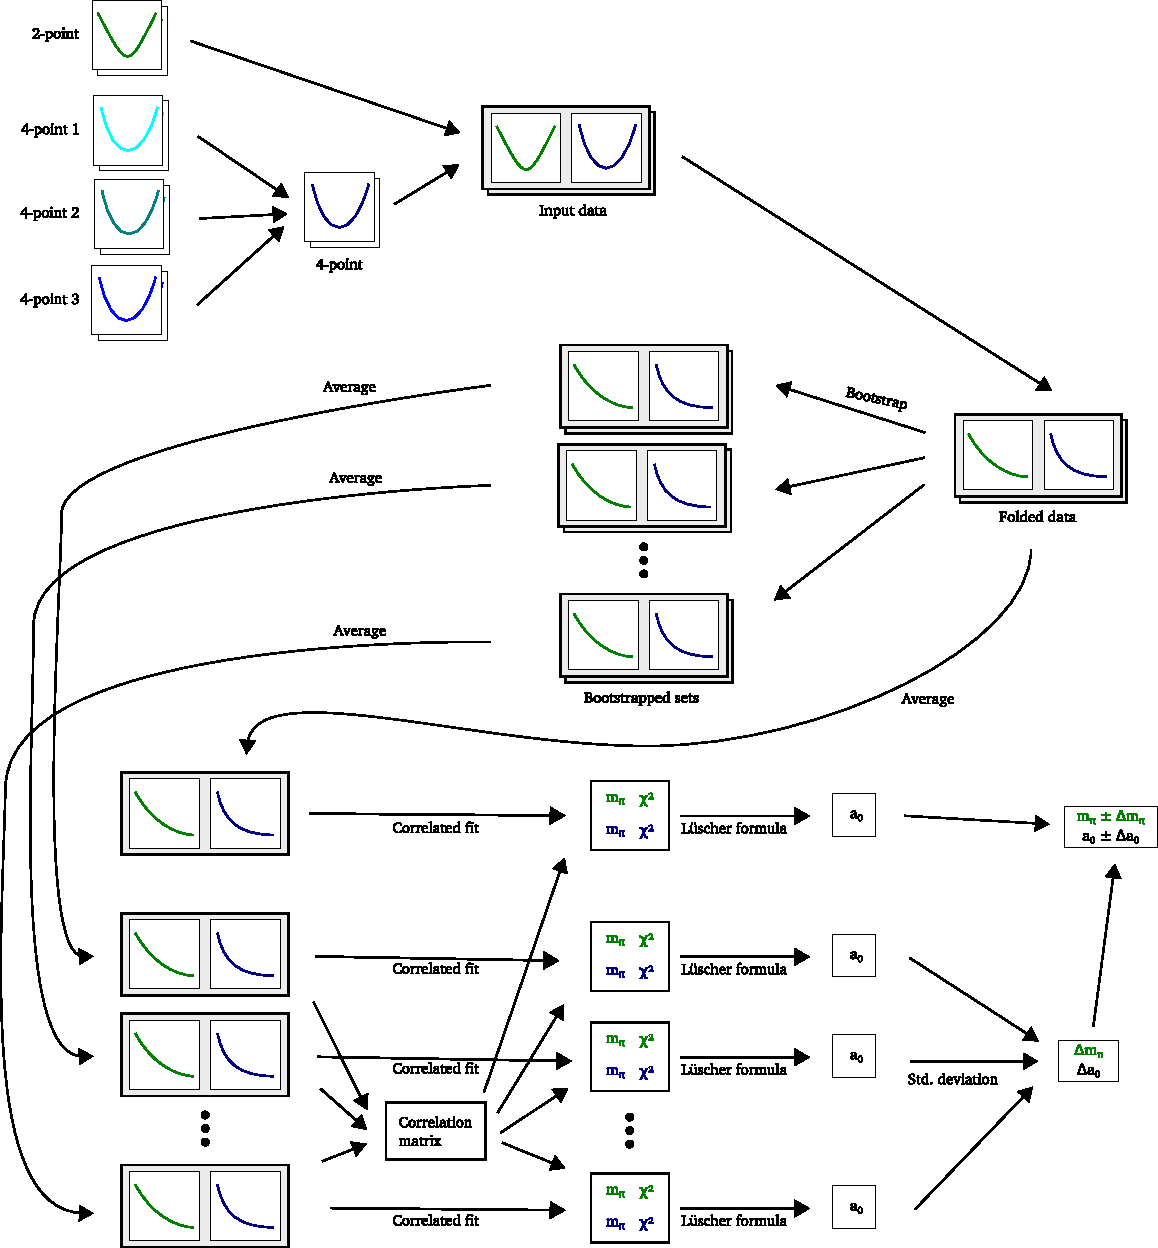
\includegraphics[width=\linewidth]{sketches/Zeichnung.pdf}
    \caption{%
        Data flow in the analysis. The first step is the import of the data,
        which is covered in Section~\ref{sec:import}. The two and four point
        functions are combined into pairs for each configuration. The data is
        then folded in half. The bootstrap step is covered in
        Section~\ref{sec:bootstrap}. Then a correlated fit is performed, see
        Section~\ref{sec:correlated_fit} for details. The second to last step
        is the application of Lüscher's formula, see
        Section~\ref{sec:scattering_length}. The results are shown in
        Section~\ref{sec:results}.
    }
    \label{fig:analysis-flow}
\end{figure}

\subsection{Import data}
\label{sec:import}

The data that I was given is organized in different ensembles (like A30.32,
A100.24) as mentioned in the introduction. For each ensemble, multiple
configurations were simulated. The output of each configuration is one
two-point correlation function $C_\piup(t)$ and three four-point correlation
functions $C_{\piup\piup}^{(i)}(t)$. Those three different contractions are
combined into a single $\piup\piup$-correlation function:
\begin{equation}
    C_{\piup\piup}(t) = C_{\piup\piup}^{(1)}(t) + C_{\piup\piup}^{(2)}(t)
    - 2 C_{\piup\piup}^{(3)}(t).
\end{equation}

Some of the ensembles had multiple versions of the data in it. I analyzed all
of them sorted by file name. In the tables, you will find the ensembles
multiple times, those are the different versions.

The number of configurations in each ensemble is called $N$.

In both space and time, the lattice used in the computation has periodic
boundary conditions. The spatial lattice extent is called $L$, the temporal one
$T$. This leads to a symmetry where the time slices $t$ and $T-t$ closely
related. The correlation functions $C(t)$ with $t = |t_1 - t_2|$ are symmetric
in $t_1$ and $t_2$, such that only the data in the interval $[0, T/2]$ carries
independent information. Before starting any other calculations with the data,
it is folded in half and averaged. The data then looks like in
Figure~\ref{fig:folded} which appears laster on.

\subsection{Bootstrap}
\label{sec:bootstrap}

All error estimation is done with the bootstrap method. One other known method
to compute errors is the Gaussian error propagation. This method involves
computing derivatives of the functions applied to the data, which can be either
numerically unstable or just not really applicable: How does the variance of
the mean change when you change the input data?

In order to get rid of all those problems at the same time one does a meta
analysis of the data itself. To get back to the example of the mean, let $X$ be
the set of $N$ data points ($x_i \in \R$). Then the estimator of the mean
$\bar\mu$ can be computed directly from $X$. Now $R$ bootstrap samples $X^r$
(upper index, no power) are computed from the set by randomly selecting $N$
elements from $X$ and putting them into $X^r$. Since $X$ is sampled from the
original distribution, it resembles the original distribution as good as it can
with only $N$ elements. $X^r$ therefore is sampled from an approximation of the
original distribution. Then the estimators for the means $\bar\mu^r$ are
computed from the bootstrapped sets. The mean of all the $\bar\mu^r$ should
give $\bar\mu$, which was computed from the original data. The error estimate
is then the standard deviation of all the $\bar\mu^r$.
\parencite[Slide~5]{Oser/Bootstrap}

The number of bootstrap samples $R$ was set to $R = 3N$ for each ensemble.

\subsection{Correlated fit}
\label{sec:correlated_fit}

The pion masses are contained in the correlation functions in the form of an
exponential decay constant. Since time is periodic in this simulation, the
correlation function is also periodic with the temporal lattice extent $T$.
Therefore, the expectation is not a simple exponential decay, $\exp(-\lambda
t)$, but a cosh-like function. The four-point functions also have a constant
contribution due to the finite lattice extent. For both two and four point
functions, the functions that I fitted to the folded data with parameters $\vec
\lambda$ are:
\begin{equation}
    \label{eq:fit2}
    m_\piup(t, \lambda) = \lambda_1 \sbr{\exp(-\lambda_2 t) + \exp(-\lambda_2
    [T - t])}
\end{equation}
and
\begin{equation}
    \label{eq:fit4}
    m_{\piup\piup}(t, \lambda) = \lambda_1 \sbr{\exp(-\lambda_2 t) + \exp(-\lambda_2
    [T - t])} + \lambda_3.
\end{equation}
The parameter $\lambda_3$ is a lattice artifact that will vanish for $L \to
\infty$.

The folded correlation functions with the fit functions are shown in
Figure~\ref{fig:folded}.

\begin{figure}[htbp]
    \centering
    \begin{minipage}[c]{0.49\linewidth}
        \centering
        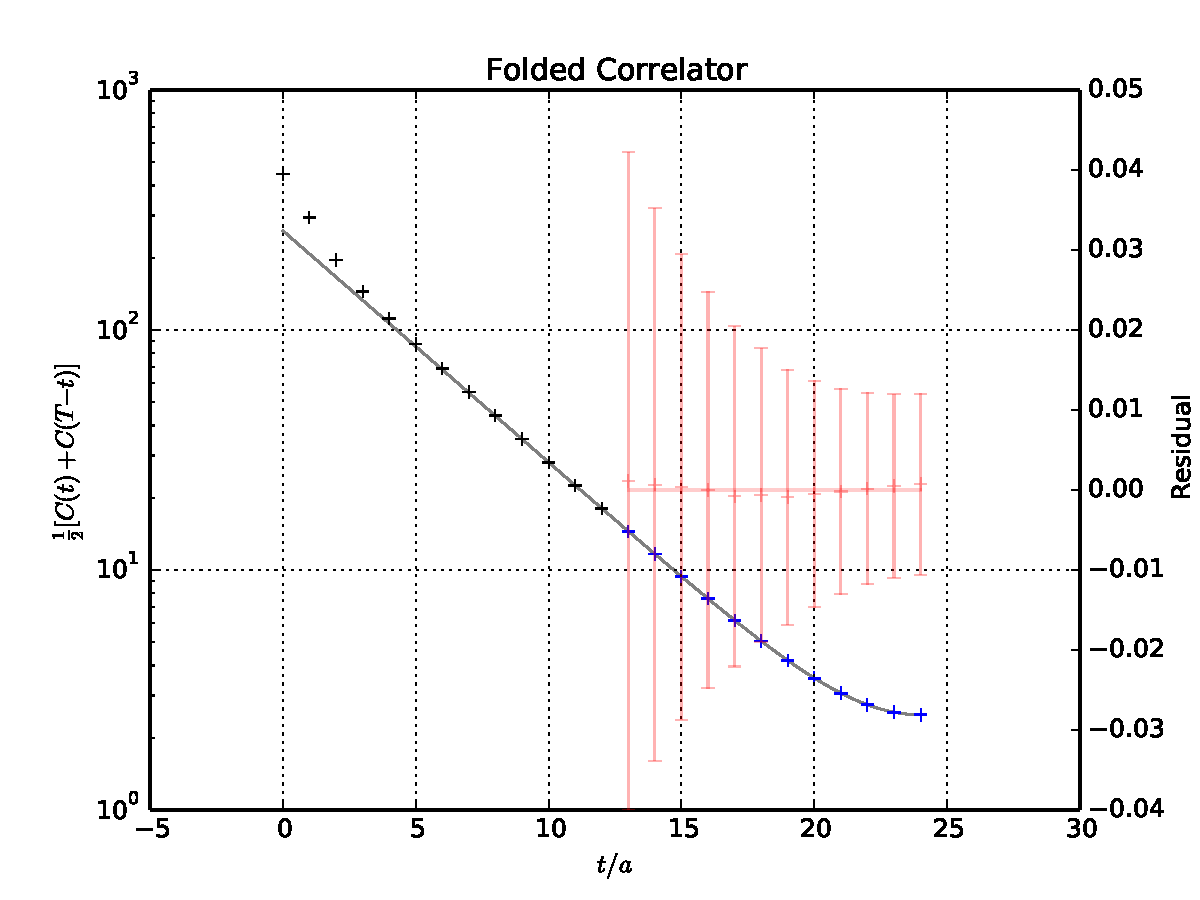
\includegraphics[width=\linewidth]{plots/A100_24_L24_T48_beta190_mul0100_musig150_mudel190_kappa1632550__ev120__TB2_SO_LI6_new_c2_folded.pdf}
    \end{minipage}
    \hfill
    \begin{minipage}[c]{0.49\linewidth}
        \centering
        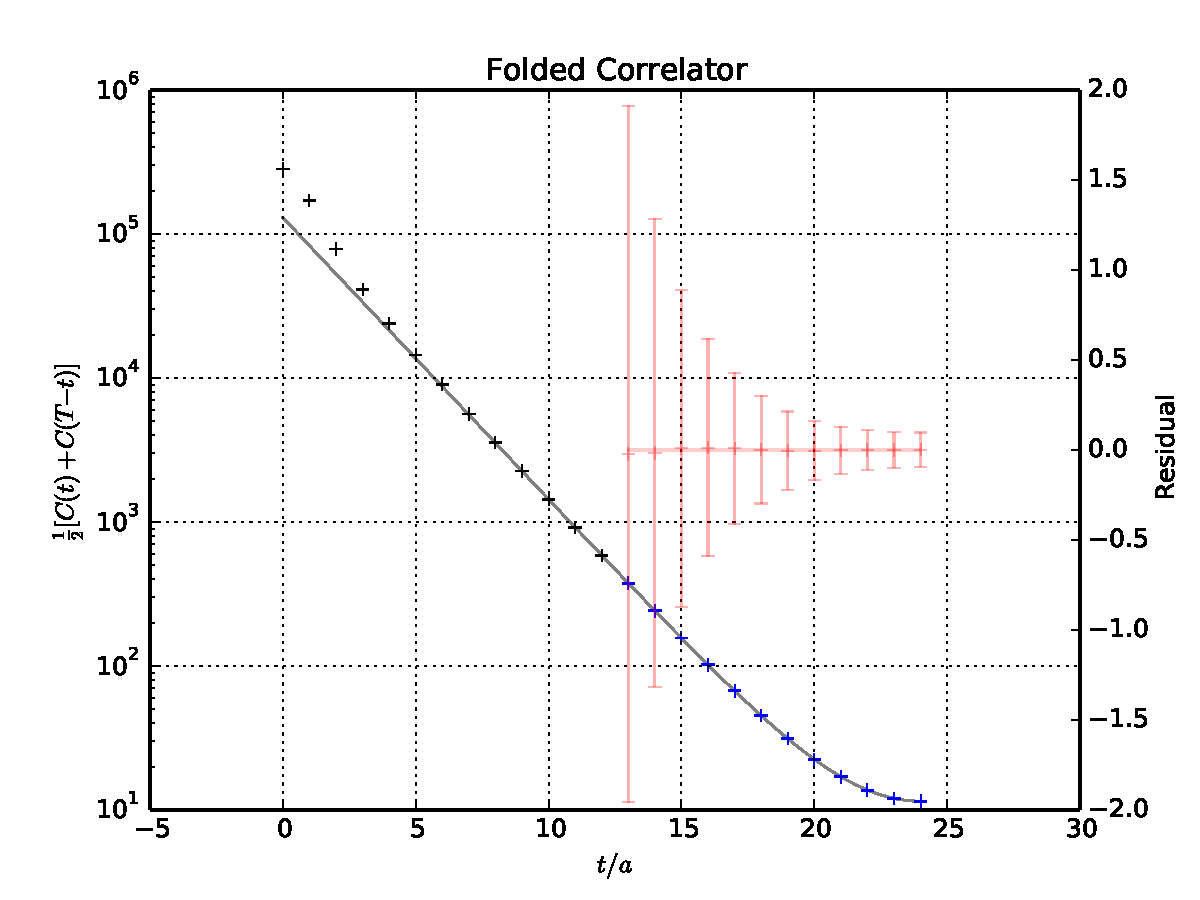
\includegraphics[width=\linewidth]{plots/A100_24_L24_T48_beta190_mul0100_musig150_mudel190_kappa1632550__ev120__TB2_SO_LI6_new_c4_folded.pdf}
    \end{minipage}
    \caption{%
        Folded correlation functions with cosh-like fit function. On the left
        side, the two point function is shown using a logarithmic ordinate
        scale. The four point function is shown on the right. Only the blue
        data points were used for fitting. The right ordinate shows the
        residuals in great magnification (red). One can see that the errors
        seem way too large compared to the residuals. This is a result of the
        autocorrelation of the data points.
    }
    \label{fig:folded}
\end{figure}

The correlation functions themselves are highly correlated with respect to
time. Therefore, a regular least squared fit would give a $\chi^2$ that would
be way too low for the assumed degrees of freedom. The $p$-values usually end
up around 1, which does not imply a perfect fit but rather that the data fits
the model \emph{too well}. This, in turn, means that errors and residuals are
over-estimated with the given model. A different model is called for: the
correlated fit.

For the correlated fit, a new likelihood function is needed. I chose to keep
the falling exponential likelihood function but incorporate the correlation
into the $\chi^2$. First, a correlation matrix $\tens C$ is needed, which is
computed from the $R$ bootstrap samples: \parencite[Section~2]{Michael:1994sz}
\begin{equation}
    \label{eq:correlation_matrix}
    C_{ij} := \frac{1}{R[R-1]} \sum_{r=1}^R
    [x_{ir} - \bar x_{iR}] [x_{jr} - \bar x_{jR}]
    \eqnsep
    \bar x_{iR} := \frac 1R \sum_{r=1}^R x_{ir}.
\end{equation}

Using this correlation matrix, a new $\chi^2$ can be defined which incorporates
the inverse correlation matrix:
\begin{equation}
    \label{eq:chisq}
    \chi^2_\text{corr} := \sum_{i, j}^T
    \left[ \bar x_{iR} - f(t_i, \lambda) \right]
    C^{-1}_{ij}
    \left[ \bar x_{jR} - f(t_j, \lambda) \right].
\end{equation}
The regular $\chi^2$ has $\tens C^{-1} = \tens 1$ and is just the sum of the
squared residuals.

In the curve fitting process, a function like
\texttt{scipy.optimize.curve\_fit} tries to find the parameters $\vec\lambda$
such that $\chi^2$ becomes minimal. In my implementation, I used the function
\texttt{scipy.optimize.leastsq} which tries to minimize the squared norm of a
vector valued function. With a Cholesky decomposition, this can be done like
so: Define the square bracket in Equation~\eqref{eq:chisq} to be the residual
vector $\vec r(\vec \lambda)$. Then the matrix multiplication can be written as
\begin{equation}
    \chi^2 = \vec r^\text T \tens C^{-1} \vec r.
\end{equation}
The Cholesky decomposition gives me $\tens C^{-1} = \tens U^\dagger \tens U$,
where $\tens U$ is a upper triangle matrix. Then I can write
\begin{equation}
    \chi^2 = [\tens U \vec r]^\dagger [\tens U \vec r]
    = \| \tens U \vec r \|^2
\end{equation}
where $\tens U \vec r$ is a vector that can be fed into
\texttt{scipy.optimize.leastsq}.
\nocite{SciPy}

As shown in Figure~\ref{fig:analysis-flow}, the correlation matrix computed from
the bootstrap samples is also used to fit the original data. Each fit yields a
value for $\mpi$ and $\mpipi$. The computed masses are shown in
Table~\ref{tab:masses}.

\subsection{Scattering length}
\label{sec:scattering_length}

There is a relation between mass difference to scattering length
\parencite[(1.3)]{luescher/volume_dependence}:
\begin{equation}
    \label{eq:luescher}
    \mpipi = 2\mpi - \frac{4 \piup a_0}{\mpi L^3} \sbr{1 + c_1 \frac{a_0}L + c_2 \frac{a_0^2}{L^2}}
    \eqnsep
    c_1 = \num{-2.837297}
    \eqnsep
    c_2 = \num{6.375183}
\end{equation}

Using the computed $\mpi$ and $\mpipi$ with Lüscher's formula, I can
numerically solve for the scattering length $a_0$. In my program, I use
\texttt{scipy.optimize.brentq} that is based on the algorithm by Brent (1973).
The computed scattering lengths are shown in Table~\ref{tab:masses}.

Equation~\eqref{eq:luescher} can be motivated like so: Let $\hat H = \hat H_0 +
\hat V$ be the Hamiltonian for two identical particles where $\hat H_0$ is the
free Hamiltonian and $\hat V$ a spherically symmetric potential with a limited
range (or faster than $1/\sqrt r$ decay). Then the probability that the two
particles are in interaction range scales like $L^{-3}$ as this is the inverse
volume which the two particles occupy. The most prominent finite size effect
scales to the third power, all other effects can only have higher powers of
$L^{-1}$.

In the first order of the potential $V$, the ground state (all momenta are zero)
will have an energy shift proportional to $L^{-3}$
\parencite[(2.24)]{luescher/volume_dependence}:
\[
    \Deltaup E = \frac{1}{2L^3} \hat V(\vec 0, \vec 0) + \mathcal O(V^2).
\]
The scattering amplitude $T$ as well as the S-wave scattering length $a_0$ can
be expanded in powers of $\hat V$ (Born series). Using first order term from
\parencite[(2.18)]{luescher/volume_dependence}, above equation can be rewritten
with the scattering length
\parencite[(2.25)]{luescher/volume_dependence}:
\[
    \Deltaup E = - \frac{4\piup a_0}{m L^3} + \mathcal O(V^2).
\]

To first order on the potential $V$, the leading term scales with $L^{-3}$,
like in Equation~\eqref{eq:luescher}. To obtain more terms, a complete
perturbation expansion needs to be written out. That expansion will be both in
terms of $L^{-1}$ and $V$. \citeauthor{luescher/volume_dependence} then was
able to group those terms in powers of $L^{-1}$ and obtain
Equation~\eqref{eq:luescher}.

\section{Results}
\label{sec:results}

My analysis of the correlation functions gives me values for the masses of a
single pion ($\mpi$) and a pair of them ($\mpipi$). Using
Equation~\eqref{eq:luescher}, I was able to compute the S-wave scattering
length $a_0$ from the energy difference. Those values are listed in
Table~\ref{tab:masses}.

\begin{table}
    \centering
    \begin{tabular}{lSSS}
        ensemble & {$m_{\piup}$}  & {$m_{\piup\piup}$} & {$a_0$} \\
        \midrule
        A100.24 & 0.22238 +- 0.00023 & 0.45125 +- 0.00052 & -1.346 +- 0.029 \\
        A100.24 & 0.22233 +- 0.00040 & 0.45083 +- 0.00095 & -1.287 +- 0.132 \\
        A100.24 & 0.22239 +- 0.00024 & 0.45111 +- 0.00053 & -1.316 +- 0.039 \\
        A30.32  & 0.12416 +- 0.00055 & 0.25135 +- 0.00144 & -0.904 +- 0.273 \\
        A40.20  & 0.14779 +- 0.00078 & 0.31429 +- 0.00162 & -1.426 +- 0.052 \\
        A40.24  & 0.14447 +- 0.00052 & 0.29815 +- 0.00109 & -1.255 +- 0.051 \\
        A40.24  & 0.14453 +- 0.00031 & 0.29842 +- 0.00071 & -1.272 +- 0.051 \\
        A40.32  & 0.14126 +- 0.00022 & 0.28626 +- 0.00055 & -1.228 +- 0.092 \\
        A60.24  & 0.17275 +- 0.00052 & 0.35278 +- 0.00126 & -1.194 +- 0.112 \\
        A60.24  & 0.17279 +- 0.00048 & 0.35404 +- 0.00099 & -1.361 +- 0.091 \\
        A80.24  & 0.19930 +- 0.00024 & 0.40511 +- 0.00057 & -1.228 +- 0.043 \\
        B55.32  & 0.15553 +- 0.00022 & 0.31589 +- 0.00055 & -1.676 +- 0.117 \\
        D45.32  & 0.12047 +- 0.00046 & 0.25057 +- 0.00137 & -2.416 +- 0.205
    \end{tabular}
    \caption{%
        Computed masses from correlation functions. The last column shows the
        scattering length $a_0$ which is computed using Lüscher's formula,
        Equation~\eqref{eq:luescher}.
    }
    \label{tab:masses}
\end{table}

The different ensembles assume different masses for the quarks. The first
number behind the letter gives the assumed quark mass. In most cases, a lower
quark mass also yields a lower pion mass $\mpi$. Those pion masses are not
directly the physical ones, one needs to extrapolate to the physical point. The
masses and scattering lengths are given in lattice units and depends on the
lattice spacing. The product of mass and scattering length, $a_0 \mpi$, is
independent of the lattice spacing and a good measure for extrapolation.
Table~\ref{tab:computed} shows this product, as well as the decay constant.

\begin{table}
    \centering
    \begin{tabular}{lSSSS}
        ensemble & {$L$} & {$T$} & {$a_0 m_\piup$} & {$m_\piup/f_\piup$} \\
        \midrule
        A100.24 & 24 & 48 & -0.2993 +- 0.0066 & 2.77 \\
        A100.24 & 24 & 48 & -0.2862 +- 0.0292 & 2.77 \\
        A100.24 & 24 & 48 & -0.2927 +- 0.0088 & 2.77 \\
        A30.32  & 32 & 64 & -0.1122 +- 0.0339 & 1.86 \\
        A40.20  & 20 & 48 & -0.2107 +- 0.0077 & 2.11 \\
        A40.24  & 24 & 48 & -0.1813 +- 0.0074 & 2.03 \\
        A40.24  & 24 & 48 & -0.1839 +- 0.0074 & 2.03 \\
        A40.32  & 32 & 64 & -0.1735 +- 0.0131 & 2.06 \\
        A60.24  & 24 & 48 & -0.2063 +- 0.0194 & 2.32 \\
        A60.24  & 24 & 48 & -0.2351 +- 0.0157 & 2.32 \\
        A80.24  & 24 & 48 & -0.2448 +- 0.0087 & 2.55 \\
        B55.32  & 32 & 64 & -0.2607 +- 0.0182 & 2.34 \\
        D45.32  & 32 & 64 & -0.2911 +- 0.0248 & 2.49
    \end{tabular}
    \caption{%
        Lattice size of the ensembles together with computed quantities.
        These data points are also shown in Figure~\ref{fig:result}. The pion
        decay constants are taken from
        \parencite[table~1]{Knippschild/Pi_Pi_Scattering}.
    }
    \label{tab:computed}
\end{table}

The results from Table~\ref{tab:computed} are shown in Figure~\ref{fig:result}.
My data points have no marker, the reference values have a diamond marker. The
solid black line is the expectation, not a fit.

As can be seen with the comparison to the reference data, that my values are a
lot less accurate than the reference ones. For most points, my errors are a lot
larger. The statistical uncertainty on my values is high enough for them to be
compatible with the reference and expectation.

\begin{figure}[htbp]
    \centering
    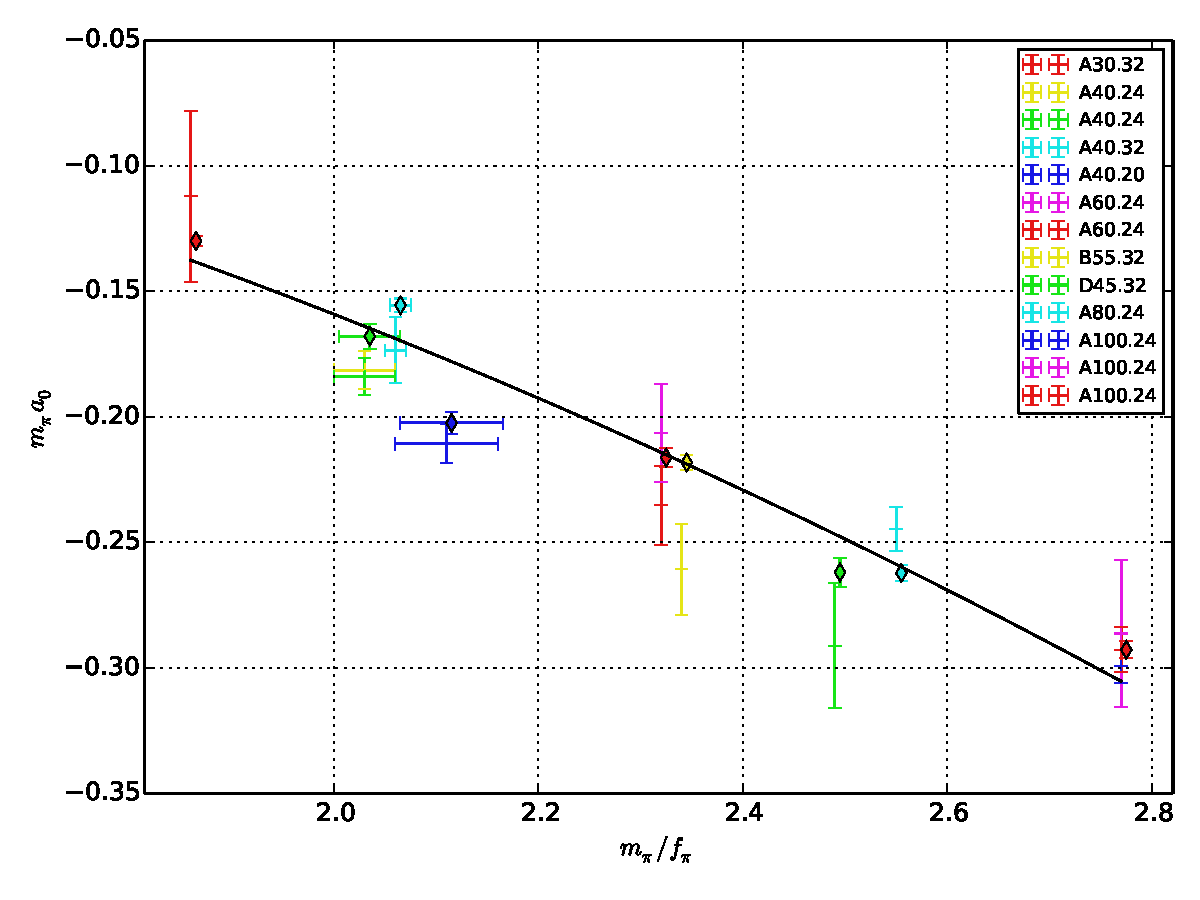
\includegraphics[width=\linewidth]{plots/result.pdf}
    \caption{%
        $\mpi a_0$ as a function of $\mpi/f_\piup$ as shown in
        Table~\ref{tab:computed}. Diamond data points are taken from draft
        paper from Carsten Urbach's workgroup. Some ensembles had multiple
        versions of the correlation functions in them, this plot shows all of
        them in lexical order of the pathname.
    }
    \label{fig:result}
\end{figure}

The range of fitting was set manually by looking at the plateau of the
effective masses. This introduces some statistical errors which cannot be
quantified with the current machinery. A way to get beyond this limitation is
to run the whole analysis with all possible fit ranges. The different result
are then weighted by the $p$-values of the respective fit.

\clearpage

\end{document}

% vim: spell spelllang=en tw=79
